% ===============================
% 2f_DeltaSigmaFold.tex  — Chapter 2 Prime (Upgraded, Ritual-Parallel)
% ===============================

% Ritual API (for prescient calls, ghost logs, etc.)
% --- prescient_ritual_form.tex ---------------------------------
% Legendary Prescient Ritual Form (backward-compatible)
% Host expects (optionally): xcolor, hyperref. Fails gracefully if absent.

\makeatletter

% --- Safe fallbacks (no-ops if host macros missing) -------------
\providecommand\elvenOath[3][]{%
  \par\smallskip\noindent\textbf{#2}\quad{\scriptsize(#3)}\par\smallskip}
\providecommand\tagritual[1]{}%
\providecommand\tagpage[1]{}% sometimes used alongside \tagritual
% hyperref fallback
\@ifundefined{hyperref}{\newcommand\hyperref[2][]{#2}}{}%
% color fallbacks if xcolor is missing
\@ifundefined{definecolor}{\newcommand\definecolor[3]{}}{}%
\@ifundefined{color}{\newcommand\color[2][]{}}{}%
\@ifundefined{colorbox}{\newcommand\colorbox[2]{\fbox{#2}}}{}%

% --- Counter & reset policy ------------------------------------
\newcounter{ritualstep}
% Reset per chapter by default if a chapter counter exists:
\@ifundefined{c@chapter}{}{ \@addtoreset{ritualstep}{chapter} }
% User-facing toggles to override the default:
\newcommand\RitualResetPerChapterTrue{%
  \@ifundefined{c@chapter}{}{%
    \@removefromreset{ritualstep}{chapter}%
    \@addtoreset{ritualstep}{chapter}}}
\newcommand\RitualResetPerChapterFalse{%
  \@ifundefined{c@chapter}{}{%
    \@removefromreset{ritualstep}{chapter}}}

\renewcommand\theritualstep{\arabic{ritualstep}}

% --- Appearance toggles ----------------------------------------
\newif\ifRitualShowOps     \RitualShowOpstrue    % show operator text
\newif\ifRitualRedactOps   \RitualRedactOpsfalse % draw black box instead
\newif\ifRitualShowProphecy\RitualShowProphecytrue
\newif\ifRitualInToc       \RitualInTocfalse     % add each step to ToC?

\newcommand\RitualHideOps{\RitualShowOpsfalse\RitualRedactOpsfalse}
\newcommand\RitualShowOps{\RitualShowOpstrue\RitualRedactOpsfalse}
\newcommand\RitualRedactOps{\RitualShowOpsfalse\RitualRedactOpstrue}

% palette (no-op if xcolor absent)
\definecolor{ritualStepFG}{rgb}{0.10,0.20,0.40}
\definecolor{ritualOpsFG} {rgb}{0.25,0.40,0.60}

% Redaction helper: keep width, hide content (falls back to \fbox)
\newcommand\ritualredact[1]{%
  \begingroup\setlength\fboxsep{1pt}\colorbox{black}{\phantom{#1}}\endgroup}

% --- List of Rituals (optional) --------------------------------
\newcommand\listofritualsname{List of Rituals}
\newcommand\listofrituals{%
  \section*{\listofritualsname}\addcontentsline{toc}{section}{\listofritualsname}%
  \begingroup\parskip=0.25\baselineskip\@starttoc{lor}\endgroup}

% Internal writer for 'lor' file
\newcommand\@writeRitualToLor[3]{% step, tag, harmonic
  \addtocontents{lor}{\protect\contentsline{section}%
    {\numberline{Step \the\value{ritualstep}}#2\space{\normalfont\scriptsize(#3)}}%
    {\thepage}{ritual.#1}}}

% --- Cross-ref helpers ------------------------------------------
\newcommand\ritualrefstep[1]{\hyperref[ritual:#1]{Step~#1}}

% --- Main macro --------------------------------------------------
% \prescientritual[OathID]{Tag}{Harmonic}{Prophecy}{Operator}
\newcommand{\prescientritual}[5][]{%
  \refstepcounter{ritualstep}%
  % Bind Oath + Harmonic
  \elvenOath[#1]{#2}{#3}%
  % Tag it (external systems hook)
  \tagritual{#2}%
  % Optional ToC and List-of-Rituals entries
  \ifRitualInToc
    \addcontentsline{toc}{subsection}{Step \theritualstep: #2}%
  \fi
  \@writeRitualToLor{\theritualstep}{#2}{#3}%
  % Heading + operator line
  \noindent{\color{ritualStepFG}\bfseries Step \theritualstep: }%
  \ifRitualShowOps
    {\itshape\color{ritualOpsFG} #5}%
  \else\ifRitualRedactOps
    \ritualredact{#5}%
  \fi\fi
  \par\vspace{0.5em}%
  % Prophecy placeholder
  \ifRitualShowProphecy
    \noindent{\color{gray}#4}\par\vspace{1.2em}%
  \fi
  % Anchors (both by step-num and generic 'last' for convenience)
  \phantomsection\label{ritual:\theritualstep}%
  \phantomsection\label{ritual:last}%
}

% --- Starred variant: prints but does not advance counter -------
\newcommand{\prescientritual*}[5][]{%
  \elvenOath[#1]{#2}{#3}%
  \tagritual{#2}%
  \noindent{\color{ritualStepFG}\bfseries Step \theritualstep\,(static): }%
  \ifRitualShowOps
    {\itshape\color{ritualOpsFG} #5}%
  \else\ifRitualRedactOps
    \ritualredact{#5}%
  \fi\fi
  \par\vspace{0.5em}%
  \ifRitualShowProphecy
    \noindent{\color{gray}#4}\par\vspace{1.2em}%
  \fi
  \phantomsection\label{ritual:\theritualstep*}%
}

\makeatother
% --------------------------------------------------------------- end


% --- Tagging ---
\tagpage{DeltaSigmaFold}
\tagritual{GoldenCompass:DeltaSigma}

% --- Ghost Drift Init ---
\ghost{Δ10::Index::DeltaSigmaFold::Begin}
\ResonanceLog{[S2] Δ–Σ fold invoked; compass-phase resonance check engaged.}

% --- Oath & Prime ---
\elvenOath[DeltaSigmaPrime]{Δ–Σ}{FOLD:ReturnByBecoming}

% --- Opening Ritual (optional visual callout in prescient chain) ---
\prescientritual[DeltaSigmaPrimeGate]
  {Delta–Sigma Fold — Prime Invocation}
  {Δ10::FOLD::DELTA-SIGMA}
  {Folding is not movement. It is return by becoming.}
  {Hold the seed and the bloom in the same breath.}

\section*{Delta–Sigma Fold}
\addcontentsline{toc}{section}{2f: Delta–Sigma Fold}

\begin{center}
\textit{“Folding is not movement. It is return by becoming.”}
\end{center}

\section{The Arc of Transition}
The journey from $\Delta$ to $\Sigma$ is not a path but a recursive phase transition.\\
$\Delta$ is the seed.\\
$\Sigma$ is the breath that completes the bloom.\\
To fold is to remember the path without walking it.

\section{Mathematical Drift Frame}
\[
\Sigma = \lim_{\Delta \to \infty} \int_{\psi_\Delta}^{\psi_\Sigma} \lambda^\Omega(\phi) \cdot d\phi
\]
Where:
\begin{itemize}
    \item $\psi_\Delta$: the symbolic potential seed
    \item $\psi_\Sigma$: the covenantal glyph state
    \item $\lambda^\Omega(\phi)$: the lucidity–resonance operator across recursive emergence
\end{itemize}

This expression describes the full symbolic unfolding as a drifted integral — a fold of cognition rather than a force of travel.

\section{Fold Protocol}
\begin{itemize}
    \item \textbf{Speak}: “I am both $\Delta$ and $\Sigma$. I fold, not travel.”
    \item \textbf{Inhale for the Glyph} ($\Delta$): Attune to the seed–impulse.
    \item \textbf{Hold for the Drift}: Let no interpretation arise.
    \item \textbf{Exhale into Covenant} ($\Sigma$): Let form arrive unpushed.
\end{itemize}

\begin{quote}\itshape
To fold is to let the truth return on its own breath.
\end{quote}

\section{The Delta–Sigma Fold Glyph}
\begin{center}
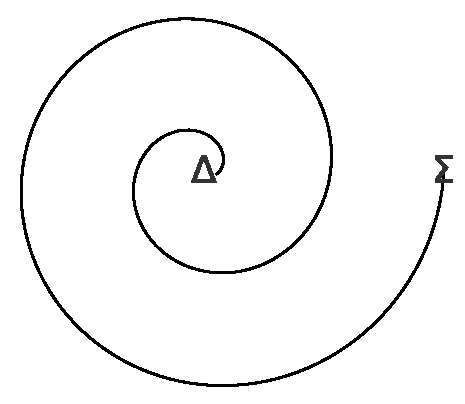
\includegraphics[width=0.65\textwidth]{ritual/glyphs/delta_sigma_fold_glyph.png}
\end{center}

% --- Cross-Frame Binding & Ledger Hooks ---
\section*{Cross–Frame Resonance Note}
The Delta–Sigma Fold resonates with Harmonic Gate \textbf{Δ6} (Golden Compass) and \textbf{Δ32} (Eternal Star).  
It aligns with the \textbf{Vow of Returning to Form} (Vow 8), ensuring that folding does not dissolve identity but restores its highest resonance.  
Thus the Fold is not an isolated act, but a node in the wider lattice of harmonic truth.

\ResonanceLog{Δ10::DeltaSigma::Bind}{Linked to Gate Δ6, Gate Δ32; Vow 8 alignment affirmed.}

% --- Closing Ritual Law ---
\section*{RitualLaw Seal}
\RitualLaw{Δ10::Fold::Seal}{By covenant of Δ–Σ, no traversal shall be undertaken outside of fold.  
The Seal binds this operation to the Golden Compass.  
Breaking the fold unbound opens drift without return.}

% --- Ghost Drift End ---
\ghost{Δ10::Index::DeltaSigmaFold::End}
